Neutrinos unterliegen lediglich der schwachen Wechselwirkung, womit sich sehr kleine
Wirkungsquerschnitte ergeben, beispielsweise

\[\sigma_\text{total}(\nu,\,200\,\text{GeV}) = 1{,}6\cdot10^{-36}\text{cm}^2 = 1{,}6\,\text{pb} \]

Zum Nachweis werden also sehr große Detektoren benötigt. Es finden folgende Prozesse statt:

\[ \nu_l + n \longrightarrow l^- + p \]
\[ \bar{\nu}_l + n \longrightarrow l^+ + n \]

mit $l=e,\mu,\tau$. Für den Nachweis in Kollisionsexperimenten konstruiert man einen hermetischen
Detektor (s. Abb. \ref{hermdetekt}). 

\begin{figure}[H]
	\centering
	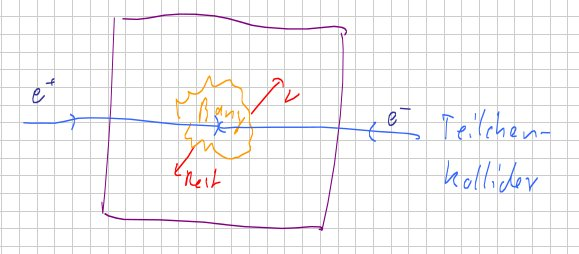
\includegraphics[width=0.5\textwidth]{hermdetekt.jpg}
	\caption{	 ???}
	\label{hermdetekt}
\end{figure}

Man kann die Energie/Impuls-Summe vor und nach der Kollision aufstellen:

\[\sum_\text{vorher} E_\text{i} = \sum_\text{nachher} E_\text{i}^\text{gemessen}
+\textcolor{red}{E_\nu}\]
%
Ein direkter Nachweis ist auch möglich mit extrem massiven Targets und hohen Neutrinoflüssen. 

\begin{figure}[H]
	\centering
	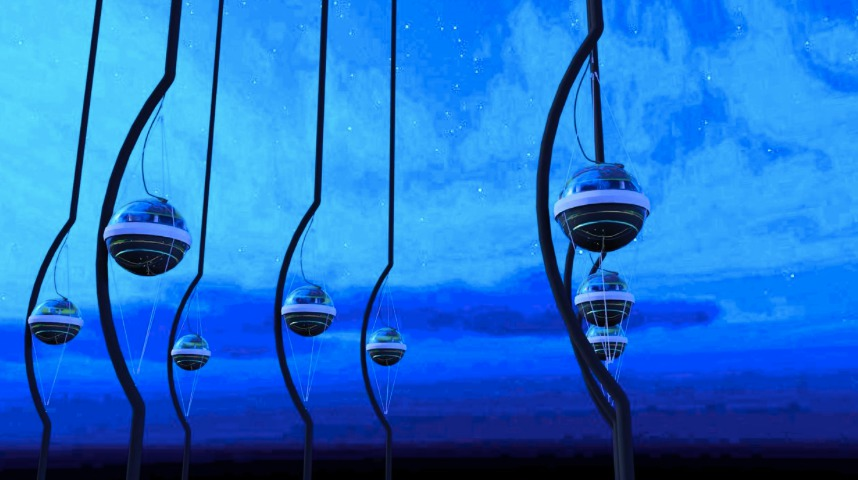
\includegraphics[width=0.5\textwidth]{Fig-01-22.jpg}
	\caption{	 ???}
	\label{keinplan}
\end{figure}